\everymath{\displaystyle}
\documentclass{beamer}
% \documentclass[handout]{beamer}

%\usepackage[pdftex]{color,graphicx}
\usepackage{amsmath,amssymb,amsfonts}

\mode<presentation>
{
  % \usetheme{Darmstadt}
  % \usetheme[hideothersubsections]{Hannover}
  % \usetheme[hideothersubsections]{Goettingen}
  \usetheme[hideothersubsections, right]{Berkeley}

  \usecolortheme{seahorse}
  % \usecolortheme{dolphin}
  \usecolortheme{rose}
  % \usecolortheme{orchid}

  \useinnertheme[shadow]{rounded}

  % \setbeamercovered{transparent}
  \setbeamercovered{invisible}
  % or whatever (possibly just delete it)
}

\mode<handout>{
  \setbeamercolor{background canvas}{bg=black!5}
  \usepackage{pgfpages}
  \pgfpagesuselayout{4 on 1}[a4paper,border shrink=5mm, landscape]
}

\usepackage[brazilian]{babel}
% or whatever

% \usepackage[latin1]{inputenc}
\usepackage[utf8]{inputenc}
% or whatever

\usepackage{times}
%\usepackage[T1]{fontenc}
% Or whatever. Note that the encoding and the font should match. If T1
% does not look nice, try deleting the line with the fontenc.


\title%[] % (optional, use only with long paper titles)
{Comparação de dois grupos (quantitativo)}

\subtitle
{Testes para médias} % (optional)

\author%[] % (optional, use only with lots of authors)
{Felipe Figueiredo}% \and S.~Another\inst{2}}
% - Use the \inst{?} command only if the authors have different
%   affiliation.

\institute[INTO] % (optional, but mostly needed)
{Instituto Nacional de Traumatologia e Ortopedia
}
  % \inst{1}%
  % Department of Computer Science\\
  % University of Somewhere
  % \and
  % \inst{2}%
  % Department of Theoretical Philosophy\\
  % University of Elsewhere}
% - Use the \inst command only if there are several affiliations.
% - Keep it simple, no one is interested in your street address.

\date%[] % (optional)
{}

% \subject{Talks}
% This is only inserted into the PDF information catalog. Can be left
% out. 



% If you have a file called "university-logo-filename.xxx", where xxx
% is a graphic format that can be processed by latex or pdflatex,
% resp., then you can add a logo as follows:

\pgfdeclareimage[height=1.6cm]{university-logo}{../logo}
\logo{\pgfuseimage{university-logo}}



% Delete this, if you do not want the table of contents to pop up at
% the beginning of each subsection:
\AtBeginSubsection[]
%\AtBeginSection[]
{
  \begin{frame}<beamer>{Sumário}
    \tableofcontents[currentsection,currentsubsection]
  \end{frame}
}


% If you wish to uncover everything in a step-wise fashion, uncomment
% the following command: 

% \beamerdefaultoverlayspecification{<+->}


\begin{document}

\begin{frame}
  \titlepage
\end{frame}

\begin{frame}{Sumário}
  \tableofcontents
  % You might wish to add the option [pausesections]
\end{frame}


%% Template
% \section{}

% \subsection{}

% \begin{frame}{}
%   \begin{itemize}
%   \item 
%   \end{itemize}
% \end{frame}

% \begin{frame}
%   \begin{columns}
%     \begin{column}{5cm}
%     \end{column}
%     \begin{column}{5cm}
%     \end{column}
%   \end{columns}
% \end{frame}

% \begin{frame}{}
%   \includegraphics[height=0.4\textheight]{file1}
%   \includegraphics[height=0.4\textheight]{file2}
%   \includegraphics[height=0.4\textheight]{file3}
%   \begin{figure}
%     \caption{}
%   \end{figure}
% \end{frame}

% \begin{frame}{}
%   \begin{definition}
%   \end{definition}
%   \begin{example}
%   \end{example}
%   \begin{block}{Exercício}
%   \end{block}
% \end{frame}

\section{Discussão da aula passada}

\subsection{Discussão da aula passada}

\begin{frame}{Discussão da aula passada}
  \begin{block}{}
    Discussão da leitura obrigatória da aula passada
  \end{block}
\end{frame}

\section{Revisão}

\subsection{Revisão}

\begin{frame}{Revisão: hipótese nula}
  \begin{block}{Conceito da hipótese nula}
    \begin{center}
      {\bf A hipótese de que não há efeito no tratamento.}
    \end{center}

    \bigskip
    \small
    O objetivo do estudo é providenciar evidências suficientes para rejeitar esta hipótese, ``provando'' assim a eficácia do tratamento.
  \end{block}
  \begin{exampleblock}{Exemplo}
    \small
    {\bf Hipótese do estudo:} um certo tratamento de fisioterapia diminui o tempo de recuperação após uma artroplastia total do joelho.

    \bigskip
    {\bf Hipótese nula:} não há alteração no tempo de recuperação.
  \end{exampleblock}
\end{frame}

\begin{frame}{Revisão: p-valor}
  \begin{block}{Conceito do p-valor}
    Assumindo que não há efeito real (hipótese nula), e você observou uma aparente diferença...

    \bigskip
    \begin{block}{}
      ... qual é a probabilidade de você ter observado essa diferença ao acaso?
    \end{block}
  \end{block}
\end{frame}

\begin{frame}{Revisão: p-valor}
\begin{block}{Interpretação do p-valor}
  \begin{itemize}
    \small
  \item Um valor pequeno para o p-valor (tipicamente $p \le 0.05$)
    representa forte evidência para rejeitar a hipótese nula, então
    deve-se rejeitá-la.
  \item Um valor alto para o p-valor (tipicamente $p \ge 0.05$)
    representa pouca evidência contra a hipótese nula, então não se
    deve rejeitá-la
  \item Um valor próximo do ponto de corte ($0.05$) é considerado
    marginal, portanto ``qualquer decisão pode ser tomada''. Sempre
    apresente seu p-valor para que o leitor possa tirar suas próprias
    conclusões.
  \end{itemize}
\end{block}
Fonte: Rumsey, D. (Statistics for Dummies, 2nd ed.)
\end{frame}

\section{Testes paramétricos para médias}

\begin{frame}{Testes estatísticos}
  Testes estatísticos sempre seguem o mesmo roteiro
  \begin{enumerate}
  \small
  \item A região crítica é escolhida (bilateral ou unilateral)?
  \item As estatísticas sumárias são calculadas a partir da amostra
  \item Estas são usadas para calcular uma estatística de teste
  \item O valor da estatística de teste é o critério de decisão:
    \begin{itemize}
    \item Pode ser comparado com um valor crítico, da distribuição de probabilidades; OU
    \item {\bf A estatística de teste é usada para o cálculo do p-valor, e este é usado como critério}
    \end{itemize}
  \end{enumerate}
\end{frame}

\begin{frame}{Testes paramétricos}
  \begin{itemize}
  \item Existe uma infinidade de testes estatísticos (cada qual com sua hipótese nula)
  \item São divididos em dois grandes grupos: paramétricos e não paramétricos
  \item Os testes paramétricos assumem que a amostra vem de uma \alert{distribuição Normal}
  \item Os testes não-paramétricos não presumem nenhuma forma para a distribuição dos dados
  \end{itemize}
  \begin{block}{Atenção}
    Esta é uma escolha metodológica fundamental na análise, como veremos no futuro.
  \end{block}
\end{frame}

\begin{frame}{Testes paramétricos}
  \begin{itemize}
  \item Os testes paramétricos assumem que a amostra vem de uma \alert{distribuição Normal} \footnote{nunca é demais frisar}
  \item Hoje veremos o {\bf teste t} (de Student), aplicado em duas formas/contextos
  % \item Ele pode ser usado para um ou dois grupos de medições.
  \end{itemize}
\end{frame}

\subsection{Dois grupos independentes}

\begin{frame}{Premissas}
  \begin{itemize}
  \item Os dois grupos foram coletados independentemente (inter-grupo)
  \item Todas as observações em cada grupo são independentes entre si (intra-grupo)
  \item Todos os dados foram amostrados de populações Normalmente distribuídas (aprox.)
  \item O DP das duas populações são idênticos \footnote{uma violação desta premissa não é grave - buscar aproximação de Welch.}
  \end{itemize}
\end{frame}

\begin{frame}{}
  \begin{block}{O teste t de Student}
      Assumindo duas populações Normais com DPs semelhantes, o teste t pode detectar diferença nas médias das populações.
  \end{block}
\end{frame}

\begin{frame}{Exemplo 1}
  \begin{exampleblock}{Exemplo 23.2}
    \small
    Motulsky, {\em et al.} (1983) investigaram se pessoas com hipertensão tem alteração nos níveis de receptores adrenérgicos $\alpha_2$ em suas plaquetas.

    \bigskip
    {\footnotesize
      Selecionaram 18 homens hipertensos, e 17 controles da mesma faixa etária.
      Os resultados estão descritos como média $\pm$ SEM.
    }

    \begin{exampleblock}{}
      \footnotesize
      As plaquetas dos hipertensos tiveram 257 $\pm$ 14 receptores por plaqueta.

      As plaquetas dos controles tiveram 263 $\pm$ 21 receptores por plaqueta.
    \end{exampleblock}
    \bigskip
    Os autores concluíram que não havia diferença significativa entre as médias dos grupos.
  \end{exampleblock}
\end{frame}

\begin{frame}[fragile]{Saída típica de um programa}
  \begin{exampleblock}{Teste t, amostras independentes}
    \footnotesize
\begin{verbatim}
P value and statistical significance: 
  The two-tailed P value equals 0.8116 
  By conventional criteria, this difference
 is considered to be not statistically significant. 

Confidence interval: 
  The mean of Controle minus Hipertensos equals 6.00 
  95% confidence interval of this difference:
 From -44.81 to 56.81 

Intermediate values used in calculations: 
  t = 0.2403 
  df = 33 
  standard error of difference = 24.973 
\end{verbatim}
  \end{exampleblock}
\end{frame}

% Review your data: 
%   Group	  Controle  	  Hipertensos  
% Mean	263.00	257.00
% SD	86.59	59.40
% SEM	21.00	14.00
% N	17    	18    

\begin{frame}{Quais são as variáveis?}
  \begin{block}{Interpretação típica}
    \begin{itemize}
    \item Grupo Hipertensos: contínua (mensuração)
    \item Grupo Controle: contínua (mensuração)
    \end{itemize}
  \end{block}
  \vfill
  \begin{block}{}<2>
    Ou, podemos pensar em termos de modelagem
  \end{block}
\end{frame}

\begin{frame}{Quais são as variáveis?}
  \begin{itemize}
  \item Dependente: níveis de receptores (contínua)
  \item Independente: grupo (categórica binária)
  \end{itemize}
  \vfill
  \begin{block}{Esta relação pode ser expressa como}
    \begin{displaymath}
      \text{níveis de receptores} \sim \text{grupo}
    \end{displaymath}
  \end{block}
\end{frame}

\subsection{Dois grupos pareados}

\begin{frame}{Grupos independentes x pareados}
  \begin{itemize}
  \item Assim como no cálculo de ICs, os grupos de estudo podem ser independentes ou pareados
  \item Quando são independentes, a comparação é entre as médias de ambos os grupos
  \item Quando são pareados, a comparação é entre as diferenças dos pares
  \end{itemize}
\end{frame}


\begin{frame}{Grupos pareados (revisão)}
Quando faz sentido parear indivíduos de dois grupos?
  \begin{itemize}
  \item Mensurar o \alert{mesmo} indivíduo antes e depois do procedimento
  \item Recrutamento aos pares, quando o par tem a(o) mesma(o)
    \begin{itemize}
    \item idade/faixas etária
    \item região demográfica
    \item diagnóstico
    \end{itemize}
  \item irmãos, pai/filho
  \item lateralidade (tratamento = lado E, controle = lado D)
  \end{itemize}
\end{frame}

\begin{frame}{Premissas}
  \begin{itemize}
  \item Os pares amostrados aleatoriamente de uma mesma população (ou representativa)
  \item Os participantes são pareados - o primeiro do grupo A com o primeiro do grupo B, etc.
  \item Cada par é independente de todos os outros
  \item A distribuição das diferenças, na população, é Normalmente distribuída (aprox.)
  \end{itemize}
\end{frame}

\begin{frame}{Exemplo 2}
  \begin{exampleblock}{Exercício 25.1}
    \small
    Os pesquisadores compararam o número de receptores beta-adrenérgicos nos linfócitos de um grupo de participantes, antes e após a administração de uma droga.

  \end{exampleblock}
\end{frame}

\begin{frame}[fragile]{Saída típica de um programa}
  \begin{exampleblock}{Teste t, amostras pareadas}
    \footnotesize
\begin{verbatim}
	Paired t-test

data:  Receptors by Group
t = 6.9636, df = 5, p-value = 0.000939
alternative hypothesis: true difference
 in means is not equal to 0
95 percent confidence interval:
 145.7279 316.2721
sample estimates:
mean of the differences 
                    231
\end{verbatim}
  \end{exampleblock}
\end{frame}

\begin{frame}{Quais são as variáveis?}
  \begin{itemize}
  \item Dependente: número de receptores (contínua)
  \item Independente: grupo (categórica binária)
  \end{itemize}
  \vfill
  \begin{block}{Esta relação pode ser expressa como}
    \begin{displaymath}
      \text{número de receptores} \sim \text{grupo}
    \end{displaymath}
  \end{block}
\end{frame}

\subsection{Exercício}

\begin{frame}{Exercício}
  \begin{exampleblock}{}
    \small
    Queremos avaliar a eficiência de uma nova dieta reduzida em
    gordura no tratamento de obesidade.

    \bigskip
    {\footnotesize
      Selecionamos aleatoriamente 100 pessoas obesas para o grupo 1, que receberão a dieta com pouca gordura.
      Selecionamos outras 100 pessoas obesas para o grupo 2 que receberão a mesma quantidade de comida, com proporção normal de gordura.
      O estudo durou 4 meses.
    }

    \bigskip
    \begin{exampleblock}{}
      \footnotesize
      A perda de peso média no grupo 1 foi de 9.33 lbs
      (s=4.72) e no grupo 2 foi de 7.58 lbs (s=3.90).
    \end{exampleblock}
  \end{exampleblock}
  \begin{block}{}
    Essa nova dieta é eficaz na perda de peso?
  \end{block}
  \hfill {\footnotesize Fonte: Khan Academy}
\end{frame}

\begin{frame}[label=perguntas]{Perguntas}
  \begin{enumerate}
  \item Para este estudo, qual dos dois testes é o mais apropriado?
  \item Qual é a hipótese nula?
  \item Qual é a hipótese alternativa?
  \item O que você usaria como critério de decisão?
  \item Qual é o resultado?
  \item Qual é a conclusão?
  \item O que significam valores negativos neste caso?
  \end{enumerate}
\end{frame}

\begin{frame}{Visualização (independentes)}
  \begin{center}
    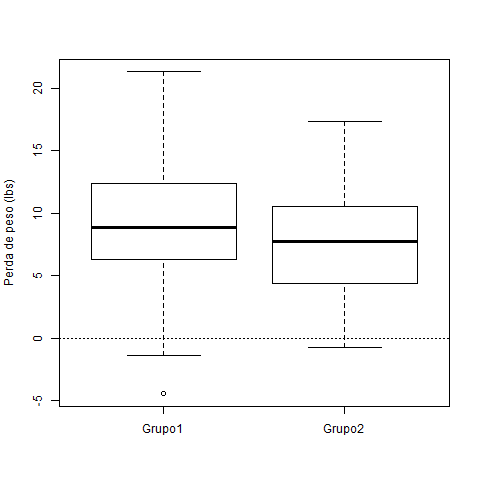
\includegraphics[height=\textheight]{Cap23-25/obesidade-independentes}
  \end{center}
\end{frame}

\begin{frame}{Visualização (pareados)}
  \begin{center}
    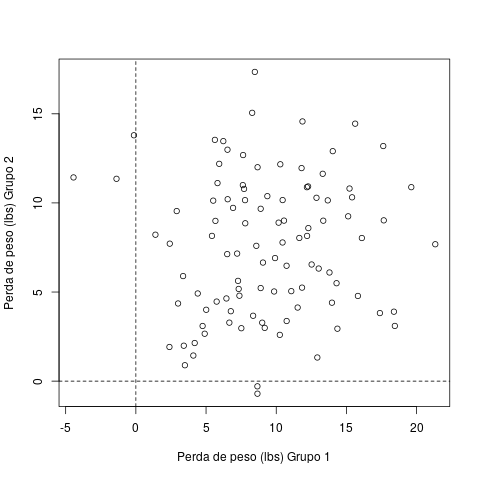
\includegraphics[height=\textheight]{Cap23-25/obesidade-pareadas}
  \end{center}
\end{frame}

\againframe{perguntas}

\begin{frame}[fragile, label=t-indep]{Saída típica de um programa}
  \begin{block}{Teste t, amostras independentes}
    \footnotesize
    \begin{verbatim}
	Two Sample t-test

data:  Perda by Grupo
t = 2.871, df = 198, p-value = 0.004537
alternative hypothesis: true difference
 in means is not equal to 0
95 percent confidence interval:
 0.5506833 2.9667462
sample estimates:
mean in group Grupo1 mean in group Grupo2 
            9.334005             7.575291 
\end{verbatim}
  \end{block}
\end{frame}

\begin{frame}[fragile]{Saída típica de um programa}
  \begin{block}{Teste t, amostras pareadas}
    \footnotesize
    \begin{verbatim}
	Paired t-test

data:  Perda by Grupo
t = 2.9545, df = 99, p-value = 0.003913
alternative hypothesis: true difference
 in means is not equal to 0
95 percent confidence interval:
 0.5775744 2.9398551
sample estimates:
mean of the differences 
               1.758715
\end{verbatim}
  \end{block}
\end{frame}

\againframe{perguntas}

\begin{frame}{}
  \begin{block}{Pergunta}
    Todas as premissas do teste que você selecionou são satisfeitas?
  \end{block}
\end{frame}

\begin{frame}{Distribuição (independentes)}
  \begin{center}
    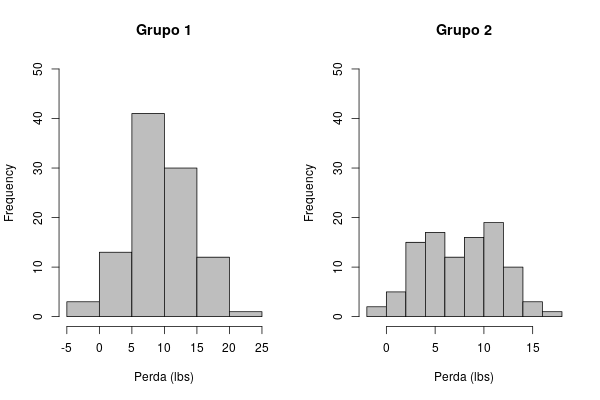
\includegraphics[height=\textheight]{Cap23-25/obesidade-hist2}
  \end{center}
\end{frame}

\begin{frame}{Distribuição (pareados)}
  \begin{center}
    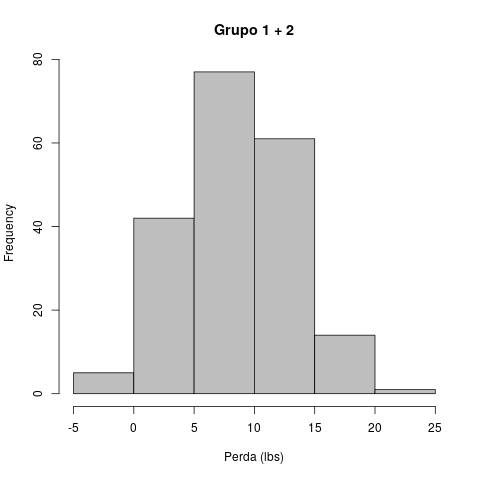
\includegraphics[height=\textheight]{Cap23-25/obesidade-hist1}
  \end{center}
\end{frame}

\begin{frame}
  \begin{block}{Caso de você tenha escolhido grupos independentes...}
    Os dois grupos tem variabilidades semelhantes?
  \end{block}
\end{frame}

\againframe{t-indep}

\begin{frame}[fragile]{Saída típica de um programa}
  \begin{block}{Teste t, amostras independentes, com correção de Welch}
    \footnotesize
\begin{verbatim}
	Welch Two Sample t-test

data:  Perda by Grupo
t = 2.871, df = 191.12, p-value = 0.004554
alternative hypothesis: true difference
 in means is not equal to 0
95 percent confidence interval:
 0.550416 2.967014
sample estimates:
mean in group Grupo1 mean in group Grupo2 
            9.334005             7.575291
\end{verbatim}
  \end{block}
\end{frame}

\begin{frame}{Quais são as variáveis?}
  \begin{block}{}
    Escreva a relação entre
    \medskip
    \begin{itemize}
    \item a variável dependente
    \item a variável independente
    \end{itemize}
  \end{block}
  \bigskip
  \begin{block}{P:}
    Qual delas varia em função da outra?
  \end{block}
\end{frame}

\subsection{Resumo}

\begin{frame}{Resumo}
  \begin{itemize}
    \small
  \item Teste paramétrico (assume dados Normalmente distribuídos)
  \item Para dois grupos independentes assume independência inter- e intra-grupo, e DPs semelhantes
  \item Para dois grupos pareados assume independência entre os pares
  \item Esta decisão \alert{não} deve ser tomada após a coleta dos dados.
  \item Variáveis:
    \begin{itemize}
    \item Dependente: contínua
    \item Independente: categórica binária (2 grupos)
    \end{itemize}
  \end{itemize}
\end{frame}

\section{Aprofundamento}

\subsection{Aprofundamento}

\begin{frame}{Aprofundamento}
  \begin{block}{Leitura obrigatória}
    \begin{itemize}
      \small
    \item Capítulo 23, pular as seções:
      \begin{itemize}
        \scriptsize
      \item Cálculo do teste t em uma tabela
      \item Cálculo do poder.
      \end{itemize}
    \item Capítulo 25, pular as seções:
      \begin{itemize}
        \scriptsize
      \item Teste t de uma razão
      \item Teste de Wilcoxon
      \end{itemize}
    \end{itemize}
  \end{block}
  \begin{block}{Exercícios selecionados}
    \footnotesize
    Não há exercícios.
  \end{block}
  \begin{block}{Leitura recomendada}
    \footnotesize
    Capítulo 25: seção teste t de uma razão (para projetos experimentais)
  \end{block}
\end{frame}

\end{document}
